\subsection{Accesul nealiniat la memoria cache}

Cea mai mare instructiune de tip SSE are 16 bytes, sau 128 de biti. Pentru fiecare operatie de tip
store/load exista 2 versiuni: prima versiune care are operatorii aliniati la 16 bytes, si cea de-a
doua versiunea care nu are operatorii aliniati.

Compilatoarele folosesc operatiile nealinitate daca nu pot garanta accesul aliniat
la memorie. Toate procesoarele de generatie anterioara, Core 2, aveau o scadere drastica a
performantei in momentul folosirii instructiunilor nealiniate fata de cele aliniate.

Problema este ca majoritatea compilatoarelor nu pot garanta aliniarea datelor in memorie si astfel
se folosesc foarte multe instructiunii nealiniate. Incepand cu arhitectura Nehalem, nu mai exista
scadere de performanta datorata folosirii instructiunilor pe date nealiniate. Astfel compilatoarele
nu vor mai fi nevoie sa alinizeze datele in memorie de teama scaderii vitezei de executie
\cite{thomadakis2011architecture}.

\subsection{Hyper-Threading}

Acesul nealiniat la memorie a fost necesar deoarece in aceasi arhitectura exista simultaneous
multithreading.

In mod normal, un procesorul nu are folosite toate modulele componente in acelasi timp, astfel ca
simultaneous multithreading foloseste aceasta ideea prin simularea a 2 nuclee virtuale folosind un
singur nucleu. Pentru acest lucru, a fost necesara marirea numarului de registrii de load de la 32
la 48 si numarul de registrii de store de la 20 la 32.

\begin{figure*}[ht] \centering
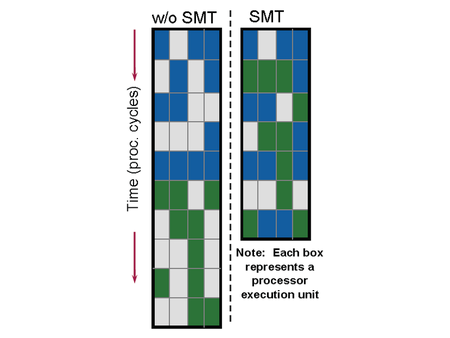
\includegraphics[width=0.6\textwidth]{img/smp.png}
\caption{Diferenta intre cu si fara Hyper-Threading } \end{figure*}

Exista arhitecturi in care se un nucleu fizic poate simula 4 nuclee virtuale, dar in cazul lui Core
i7, Intel a decis sa foloeasca doar 2 nuclee virtuale pentru fiecare nucleu fizic. Astfel in cazu
in care pe un nucleuz s-ar executa operatii cu intregi, unitatea in virgula mobile, ar putea fi
utilizata de un alt thread care ar dori sa foloseasca operatii cu numere reale \cite{semin2009inside}.


\subsection{Controlul Avansat al Consumului}

Intel Core i7 are 4 stari principale ale consumului\cite{power}.

\begin{itemize}
\item P-State - starea de performanta maxima a microprocesorului
\item T-State - starea de sleep in care microprocesorul are frecventa redusa
\item C-State - starea in care procesorul este in sleep
\item S-State - starea de sleep ale sistemului
\end{itemize}

\begin{figure*}[ht] \centering
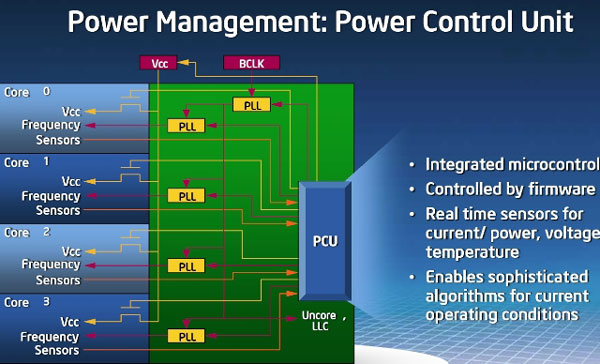
\includegraphics[width=0.6\textwidth]{img/pcu.jpg}
\caption{Unitatea de control a puterii } \end{figure*}

\subsection{Modul Turbo Boost}
Datorita existentei unui control dedicat al puterii, nucleele pot rula la frecvente independente.
In cazul in care doar 2 nuclee din 4 sunt folosite, atunci cele 2 nuclee vor putea rula la o
frecventa mai mare decat cea de baza , deoarece vor folosi puterea salvata prin inchiderea
celorlate 2 nuclee. De exemplu, daca frecventa de baza a unui procesor cu 4 nuclee este de 2,66 ghz
atunci daca maxim 2 nuclee sunt folosite, acestea vor puteea rula la o frecventa maxima de 3 ghz.

\cite{gelsinger2008intel}.

\begin{figure*}[ht] \centering
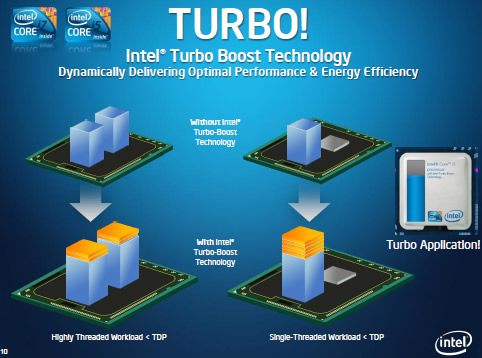
\includegraphics[width=0.6\textwidth]{img/turbo.jpg}
\caption{Exemplu de Turbo Boost } \end{figure*}


